\documentclass[
	english,
	fontsize=10pt,
	parskip=half,
	titlepage=true,
	DIV=12
]{scrartcl}

\usepackage[utf8]{inputenc}
\usepackage{babel}
\usepackage[T1]	{fontenc}
\usepackage{lmodern}
\usepackage{microtype}
\usepackage{color}
\usepackage{csquotes}
\usepackage{xspace}

\usepackage{hyperref}

\newcommand*{\tabcrlf}{\\ \hline}

\usepackage{amsmath}
\usepackage{amssymb}
\usepackage{dsfont}
\usepackage[arrowdel]{physics}
\usepackage{mathtools}
\usepackage{siunitx}

\usepackage{minted}
	\usemintedstyle{friendly}

\newcommand*{\inPy}[1]{\mintinline{python3}{#1}}
\newcommand*{\ie}{i.\,e.\xspace}
\newcommand*{\eg}{e.\,g.\xspace}

\begin{document}

\part*{Python Problems 06, Summer 2021}
Some time in 2012 I woke up on a Sunday morning with a pressing question in my head: How likely is it to randomly run into a pregnant women in different countries around the world. Needless to say I spent the rest of the day crunching numbers. You see, back in 2012, I didn't know yet how to write Code in Python.

We will tackle this problem of mine in a more efficent manner and use the module pandas to find out the \textbf{density of pregnant women in} $\mathbf{\frac{1}{\text{km}^2}}$.

\section{Data Source}
When I did this in 2012, I found out about the \emph{CIA World Factbook}\footnote{\url{https://www.cia.gov/the-world-factbook/}}. It is a freely accessible database of country profiles, maintained by the CIA and put under public domain. GitHub User TheWireMonkey\footnote{\url{https://github.com/thewiremonkey}} went through the hassle of compiling the available information into CSV files (by means of a Web Crawler, I presume), which are more easily digestible for computers than the CIA websites. You can download a compilation from October 2015 on GRIPS (file \texttt{factbook.csv-master.zip}\footnote{Original file taken from \url{https://github.com/thewiremonkey/factbook.csv}}).

Familiarize yourself with the layout of the data in this archive by opening the files within in a text editor or a spreadsheet program such as MS Excel.

You will find \texttt{CODES.md}, \texttt{NOTES.md} and \texttt{README.md}, which you can ignore (They hold complementary information for human readers).

The file \texttt{categories.csv} tells you which data are to be found in which file. Its first few lines read:
\begin{center}
\fontfamily{pcr}\selectfont
\begin{tabular}{lll}
Num & Category & Name\\
2147 & Geography & Area\\
2119 & People and Society & Population\\
2002 & People and Society & Population growth rate\\
\end{tabular}

...
\end{center}
which signifies that you'll find the population growth rates of the various countries in the file \texttt{c2002.csv} within subfolder \texttt{data}. The data in these \texttt{c\#\#\#\#.csv} files in turn look like this:
\begin{center}
\fontfamily{pcr}\selectfont
\begin{tabular}{lll}
Pos & Name & Value\\
1 & South Sudan & 4.02\\
2 & Malawi & 3.31\\
3 & Burundi & 3.27\\
\end{tabular}

...
\end{center}
\ie, in them you'll find two columns \texttt{Name} and \texttt{Value} that tell you, which country has which population growth rate. The Spreadsheets are sorted by value. If you aren't sure in which units the quantities are measured, go check out the human-readable version, \eg on \url{https://www.cia.gov/the-world-factbook/countries/germany/}. (You'll find that on that website, even more data are listed than in the CSV compilation provided).

\section{Identifying and Loading the Relevant Data Files}
To get the density of pregnant women per square kilometer, you can use this formula:
\begin{equation*}
	[\text{pregnancy-density}]
=
	\frac
		{\text{[Birth rate]}}
		{\text{[Area]}}
	\cdot
	\frac
		{\text{[Total population]}}
		{1000}
	\cdot
	\frac
		{280 \text{ days}}
		{365 \text{ days}}
\end{equation*}
(This neglects the possibilty of twins/multiplets as well as abortions and other factors, but seems fairly accurate to me.)

From this formula you can read that you'll have to load at least three files, of which you first have to identify the file name.

Write your code such that you can define a \inPy{list relevantCategories = ["Area", ...]} to the effect that a \inPy{dict filenames} is computed which holds the filenames associated with the categories in the list. Then, load the CSVs for Area, \ldots into a new \inPy{dict sources}.

\section{Consolidating Data Frames and First Computations}
Make it so that the data in \texttt{sources} gets packed together into a single \texttt{pd.DataFrame data} that can be indexed by its country name. Append the column \texttt{Pregnancy density} which should be computed according to the formula above.

You will notice that the necessary data for this computation are not available for all countries. In such a case, pandas will store \texttt{NaN} (\emph{not a number}). Get rid of these void records by using the \texttt{dropna} method.

The output of \inPy{print(data)} should look like this:
\begin{center}
	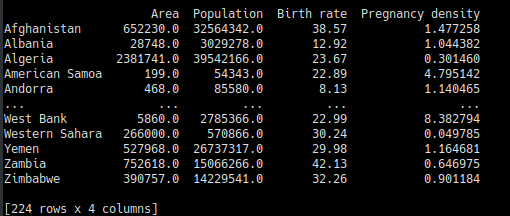
\includegraphics[width=.6\linewidth]{./DataFrame-Minimal}
\end{center}

\section{Sorting and Binning}
Sort the DataFrame by pregnancy density. Print on screen the lowest and highest pregnancy densities.

Now, find out which countries have approximately the same pregnancy density. That is, group them into bins specified by an intervall of pregnancy densities. To that end you can use \texttt{pd.cut}. Look up how that method works under \url{https://pandas.pydata.org/pandas-docs/stable/reference/api/pandas.cut.html}, or in the PDF documentation. Use 30 logarithmically spaced bins, and print on screen, how many nations fall within that bin.

Also make it so that your code shows in which bin Germany (or any country you might be interested in) falls, and which other countries are in that class.

\emph{Hint}: You will likely get empty bins, and depending on the method you choose to print them on screen, the empty bins will not be shown. My output looked like this:
\begin{center}
	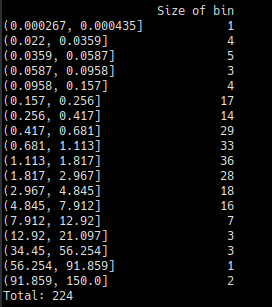
\includegraphics[width=.3\linewidth]{./Bin-Sizes}
\end{center}

\section{Data Analysis and Plots}
Reconstruct the following plot from your DataFrame:
\begin{center}
	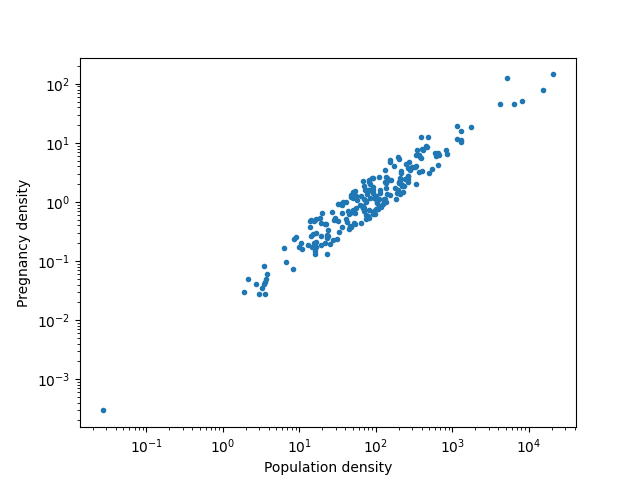
\includegraphics[width=.7\linewidth]{./PopVsPreg}
\end{center}

It shouldn't be too surprising that there is a strong correlation between overall population density and pregnancy density -- the more people there are, the more of them can be pregnant. But what is causing the spread of this plot?

Compute the \emph{normalized pregnancy density}, \ie $\frac{\text{[Pregnancy density]}}{\text{[Population density]}}$. Plot it against characteristics that you think might affect the number, like I did below:
\begin{center}
	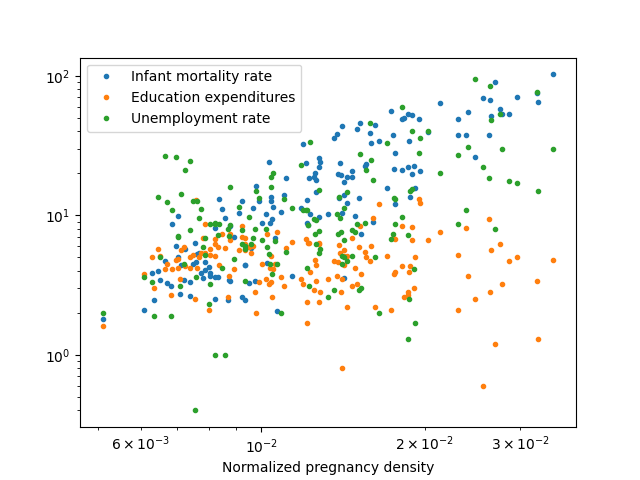
\includegraphics[width=.7\linewidth]{./DataAnalysis}
\end{center}
This plot tells us that there seems to be a strong correlation between infant mortality rate and normalized pregnancy density; a link between unemployment rate pregnancy density is debatable and education expenditure (\emph{percent} of GDP spent on education) seems to show no trend. Can you uncover any non-obvious relations? Feel free to data-nerd around, but: don't get carried away ;)

\begin{center}
	
\includegraphics[width=.9\linewidth]{./xkcd-nerdSniping}
\end{center}

\end{document}
